\chapter{Objectives and Design}

The project has a certain set of requirements that are to be satisfied, in order to accomplish it.
Here, I will provide the overview of the goals set by the project, design implementation aimed to meet those and certain properties of the problem that affected the solution.

\section{Main Objectives}

Throughout the course of project, the main aims targeted were:

\begin{enumerate}
\item {\textbf{Create a distributed version of NeMo, making it capable of scalable simulations with the use of multiple processes} (expanded in 3.2.1)}
\item {\textbf{Throughout implementation of the distributed capabilities, leave the core NeMo functionality intact - build on top} (expanded in 3.2.2)}
\item {\textbf{Implement clustering algorithm that would allow the resulting program to operate within the network capacity and distribute the workload in a more efficient manner} (expanded in 3.2.3)}
\item {\textbf{Improve the performance of large scale simulations through the use of parallel processes} (expanded in Evaluation)}
\end{enumerate}

Setting out the objectives this way helped to percieve a more detailed picture of the project as a whole and gave understanding of the set of stages that were to be accomplished in order to
make the project meet these objectives.

\section{Objective-specific Structure}

After having all of the main goals set out, it is important to get the structure of the design, with focus on satisfying these goals. In this section, the design focused on each of the features of the project will be discussed.

\subsection{Distributed Version of the Simulator}

In order to provide a more detailed picture of the distributed system, here is the set of inner classes of the NeMo core simulation classes.

\begin{figure}[h!]
\begin{center}
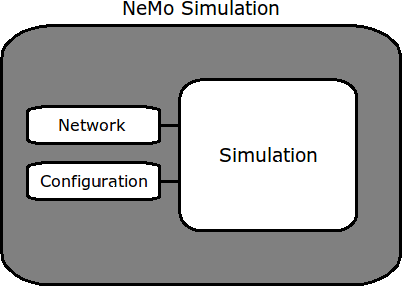
\includegraphics[scale = 0.6]{images/design/nemo_simulation_schematic.png}
\end{center}
\caption{Schematic representation of NeMo simulation}
\end{figure}

Early in the project design it became apparent from the experience from MPI examples\cite{}, that for the distributed simulation to run successfully, there has to be a hierarchy between classes - in this particular case, Master - Worker simulations. This way there would be a controller that would output the collected information, distribute the initial configuration and ensure synchronization between all of workers throughout timesteps.

Creation of the distributed system that would run the simulator could be split into 3 distinct steps:

\begin{enumerate}

\item{\textbf{Creation of fully separate homogeneous simulation}}

By accomplishment of this step, the system has to be able to run on several processes with little input from the user and no interaction between processes within simulation - in other words, several separate NeMo simulations with their own self-generated parameters, that could be started by user signal from the main process.

\begin{figure}[h!]
\begin{center}
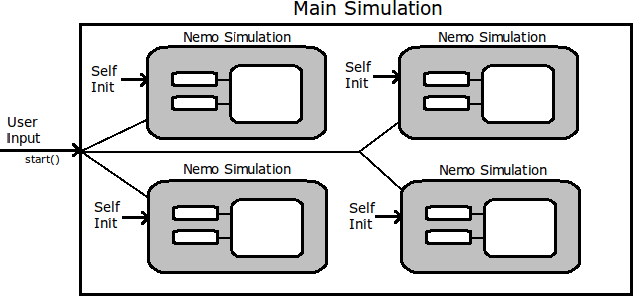
\includegraphics[scale = 0.7]{images/design/design_stage_1.png}
\end{center}
\caption{Schematic model of step 1}
\end{figure}

\item{\textbf{Integrating the initialisation parameters distribution across the network}}

After thorough research conducted into the use of MPI protocol, create a simulation that would encode and pass all the initialisation parameters to the networks - mapping, configuration, neuron and synapse data - however, still without interaction between the sub-simulations.

\begin{figure}[h!]
\begin{center}
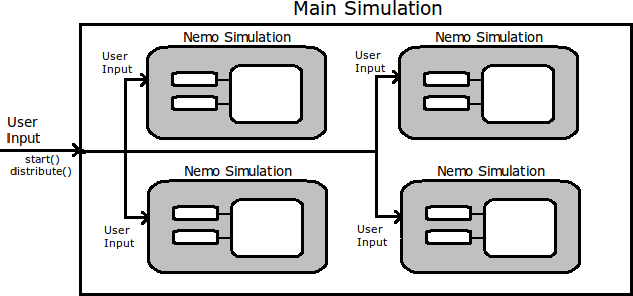
\includegraphics[scale = 0.7]{images/design/design_stage_2.png}
\end{center}
\caption{Schematic model of step 2}
\end{figure}

\item{\textbf{Implementation of the full non-constrained communication between the nodes within the network}}

Having the basic distribution system created, integrate the inter-node communication system that would allow subsystems to pass the internal spike data during simulations, while main class synchronizes the steps of all simulations by waiting for all of the communication to end, and then advancing simulation one step further.

\begin{figure}[h!]
\begin{center}
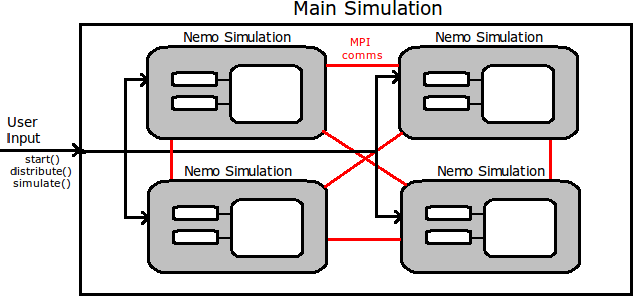
\includegraphics[scale = 0.7]{images/design/design_stage_3.png}
\end{center}
\caption{Schematic model of step 3}
\end{figure}

\end{enumerate}

Accomplishing all of these steps yields a fully working distributed implementation of the target system. It is worth noting that though this design is quite schematic, the results of the actual implementation if broken into steps were closely related to the pattern presented by this plan.

\subsection{Separation from the core NeMo System}

This section covers the structure of design that allows the distributed version be built on top of NeMo simulator without altering it.

\begin{figure}[h!]
\begin{center}
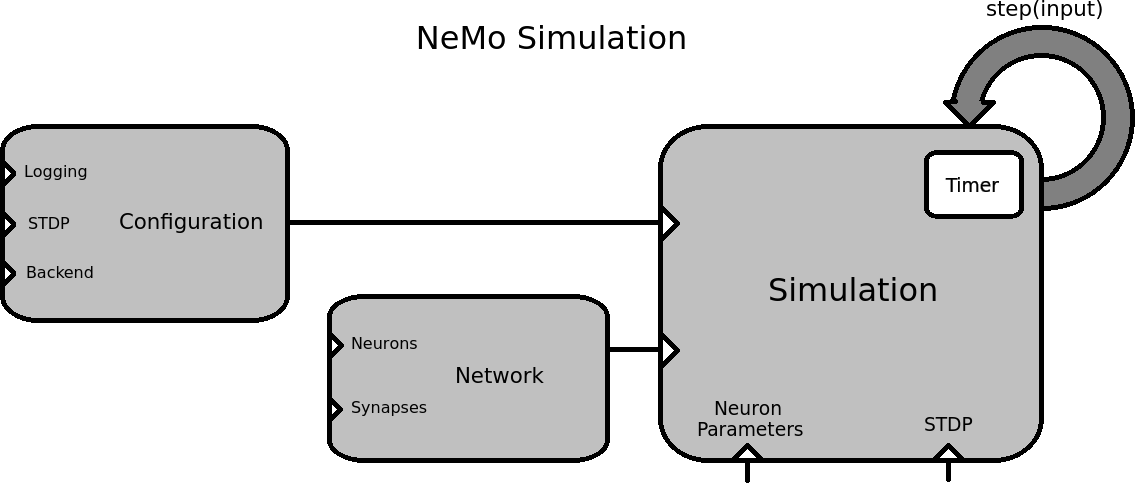
\includegraphics[scale = 0.4]{images/design/core_simulation.png}
\end{center}
\caption{NeMo core simulation design}
\end{figure}

These three classes are the core of the NeMo functionality, as they comprise all the data sets needed for the correct simulation. Therefore, in order to enable the distributed version to run separately, i.e. without interfering with the data innate to these classes, it is essential to design the system around those. In other words, the correct design must not alter internal structure of this set of classes.

In order to make the project meet this target, the structure has been developed with a strict guidance of publicly accessible properties of NeMo simulation classes. Here is the result:

\begin{figure}[h!]
\begin{center}
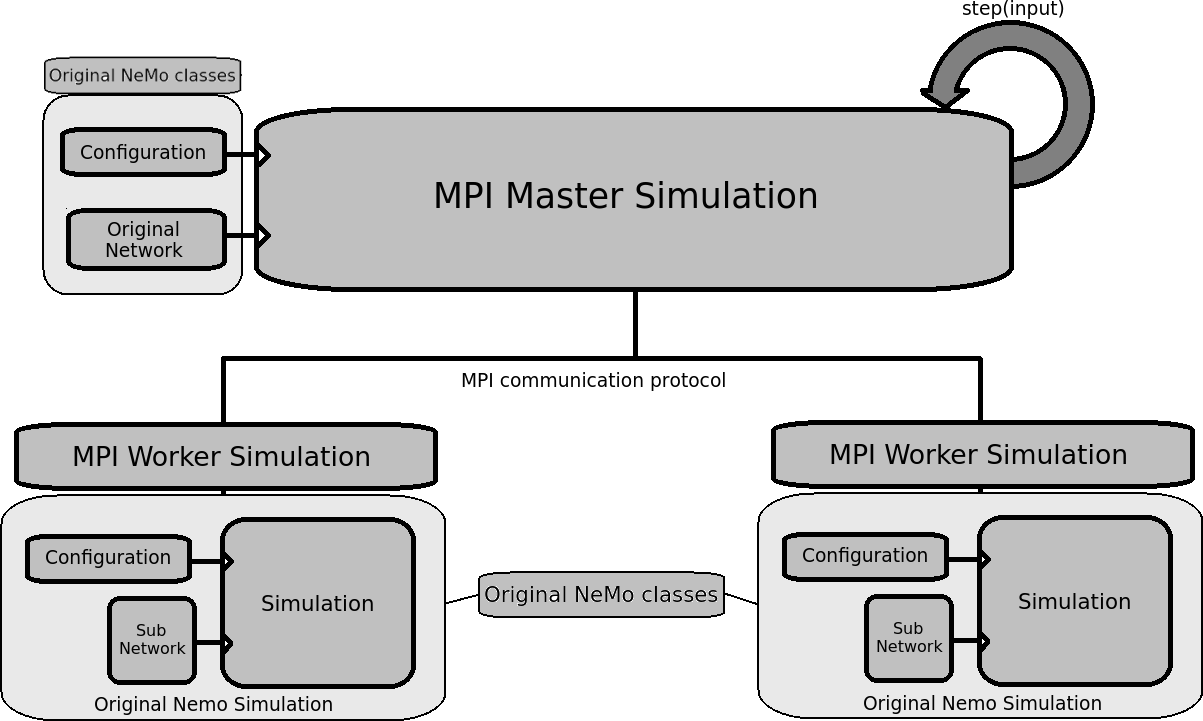
\includegraphics[scale = 0.5]{images/design/distributed_version_separated_design.png}
\end{center}
\caption{Distributed simulation design}
\end{figure}

As it can be easily observed, the design of the distributed version treats the core simulation classes as separate entities, only interacting with them through the NeMo-specified functionality and set of public methods, already present in them. To summarise, the MPI Layer wraps around the simulation classes and enables communication by passing input and output data between separate NeMo simulations.

\subsection{Cluster Mapping}

In this section, the structure of the mapper class will be discussed. The actual clustering function will be expressed in detail later, in Implementation.

Mapping as a procedure is taking place early during the simulation initialisation, therefore, it does not have strong time constraints. However, it is worth noting that it still has to abide the rule of non-interference within NeMo core functionality, as a result, collecting information only through the public methods, rather than dealing with the actual data sets.

Mapper class design has three main requirements it has to satisfy: correct implementation of mapping function, relative to the modularity of the network and number of processes it should be split between, compressibility, as the mapper is to be distributed among the worker simulations for the later use during communication, and quick to access, as its features would be needed for the communication.

\begin{figure}[h]
\begin{center}
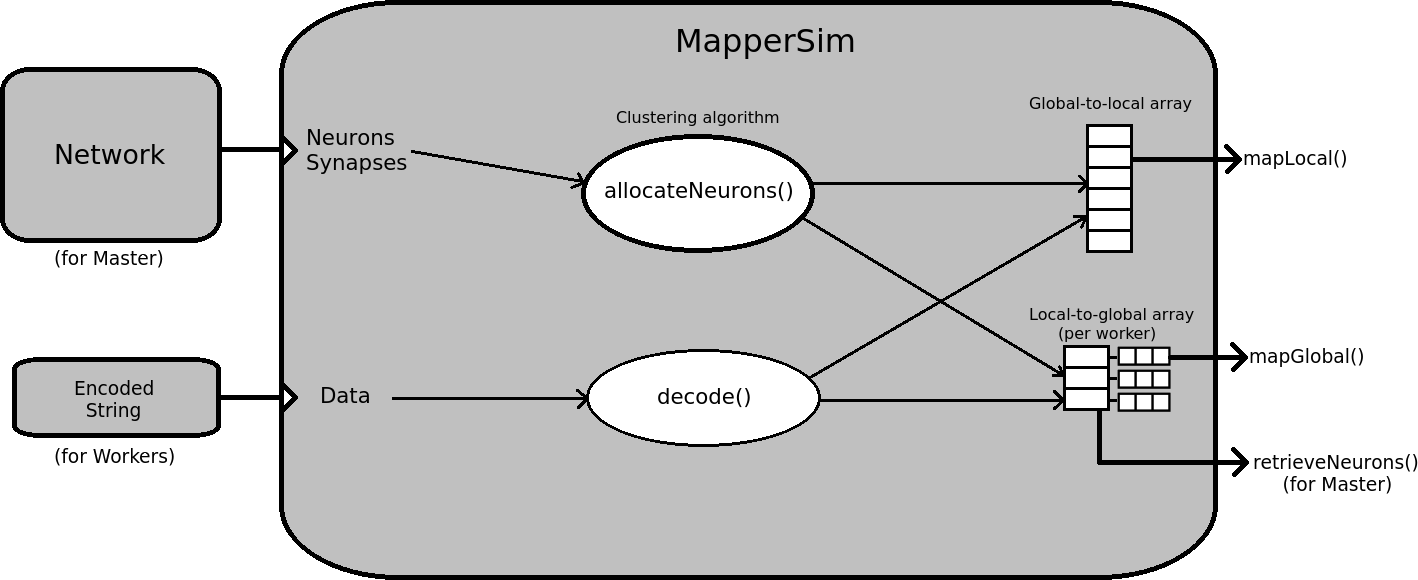
\includegraphics[scale = 0.4]{images/design/mapper_design.png}
\end{center}
\caption{Mapper class design}
\end{figure}

The core functionality of the mapper requires to have a storage for neuron global-to-local and local-to-global mappings. This is accomplished by implementing two arrays that are populated during the simulation setup stage via interaction with the NeMo network class. The choice of using arrays was made as they are easy to access and relatively simple for compression, therefore meeting two goals at once.

\section{Alternative Solutions}

Throughout the stage of designing of the distributed version, there have been several possibilities of use of alternative solutions for the given task. Here, explanation of choice made at these points will be given.

\begin{itemize}

\item{\textbf{Non-hierarchical model for distributed system}}

Non-hierarchical in this context means that there would be no division master-worker between the processes - all MPI Simulation classes would be constructed in a way to support the Master capabilities - therefore achieving maximum utilisation of available resources. This approach, however, had a big overhead in terms of synchronisation, as the step function would not be as easy to implement. Moreover, the initial split of initialisation parameters would also cause an overhead in simulation - as it would have to be done inside each Worker simulation.

Therefore, the hierarchical approach was taken further into development for its distribution and synchronisation capabilities.

\item{\textbf{Single mapper, accessible across the network}}

This solution aimed at disposing of necessity to distribute the mapper across the workers. This would save space and make simulation setup time shorter, however, a lot more network capacity would be used for queries, more time would be needed to execute those and, finally, separate mapper, being a shared resource would definitely cause a bottleneck for a parallel simulation.

Therefore, after careful consideration, this idea was discarded in favor of distributing the same mapper to all workers - and by doing this increasing the speed of simulation step communication.

\item{\textbf{Provide the inner set of variables of the network to the mapper during initialisation}}

If this step is taken, less time would be needed for mapper generation - however, this would also breach the policy of non-interference with the innate NeMo properties, by altering the adding more public internal functions.

This proposal made one of the objectives unsatisfiable, thus, was not the most preferred for the aim of the project - as a result the Mapper class was constructed to interact with the public methods of Network only.

\end{itemize}

\clearpage

\section{Final Design}

\begin{figure}[h]
\begin{center}
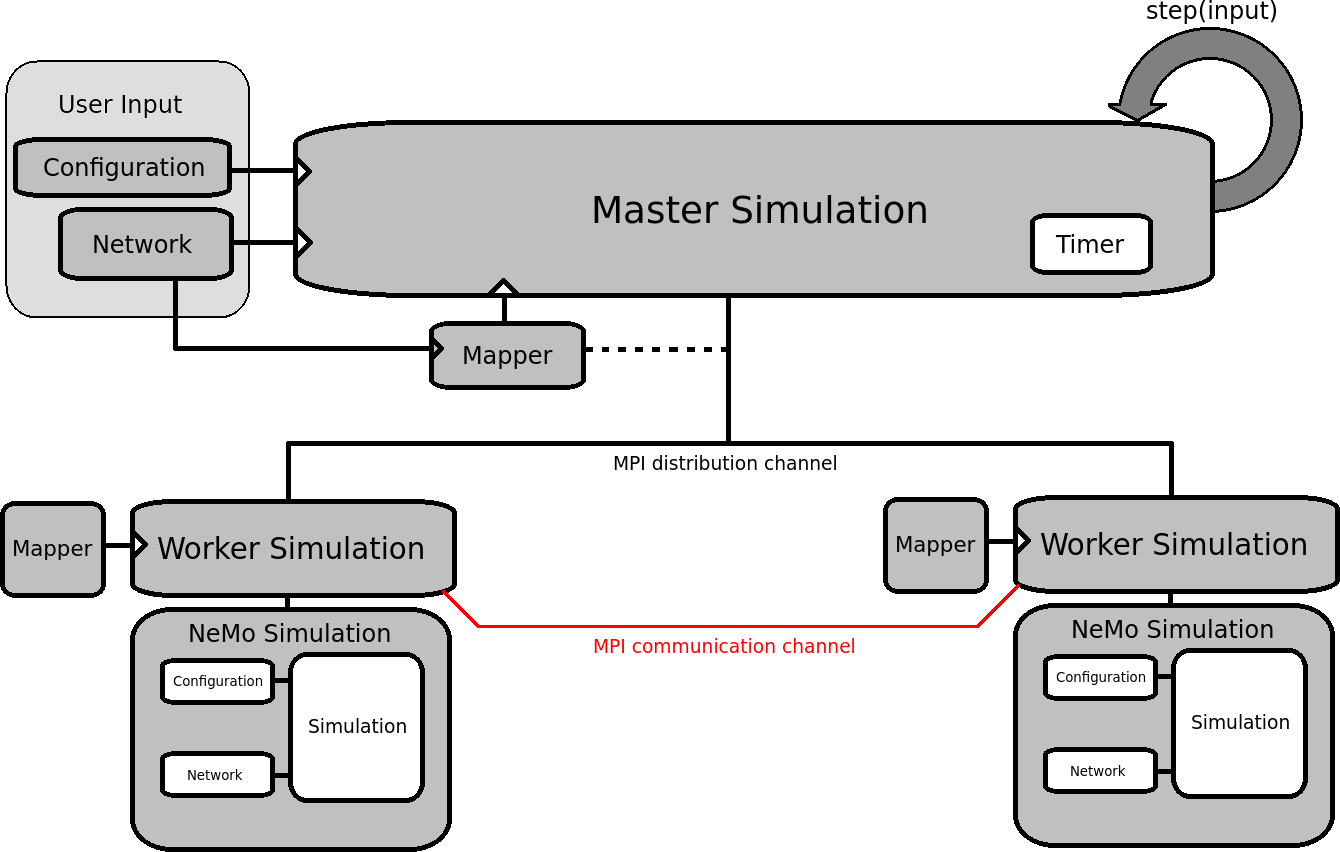
\includegraphics[scale = 0.45]{images/design/final_design.png}
\end{center}
\caption{Final project design}
\end{figure}

By comprising all of the objective-fulfilling designs from parts 3.2.1-3.2.3 into one solution, the final design of the system was built. The diagram shows the high level design structure, full properties of each part are not shown.

It has most of NeMo core functionality and provides the distributed version of simulation that could be mapped onto any number of processes. This design satisfies all of the structural requirements set by the project and, once implemented, generates the appropriate solution to the given problem.
